
\chapter{Introduction}

\label{Introduction}\emph{Ravel} is a data analysis program which
is an alternative to spreadsheets and existing business intelligence
programs (Tableau, Power BI, etc.). It has two key features that distinguish
it from all other programs in this space: 
\begin{itemize}
\item The Ravel, a visual representation of multidimensional data that is
far easier to use than Pivot Tables; and
\item Equations that are written as flowcharts, rather than the obscure
cell references of spreadsheets.
\end{itemize}
It also includes the system-dynamics engine \emph{Minsky}, which is
documented here: \ref{Introduction-Minsky}.

Unlike spreadsheets, which are fundamentally limited to two dimensions
(rows and columns), \emph{Ravel} supports an effectively unlimited
number of dimensions. \emph{Ravel}'s key feature---also called a
Ravel---is a visual tool for manipulating and analysing multidimensional
data, which can handle as many dimensions as your data contains. 

This is a blank Ravel---a Ravel with no data attached to it. The
axes are indicative examples, and will be replaced by the dimensions
of your data, once you attach a data parameter to the Ravel:

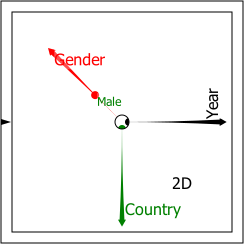
\includegraphics{images/RavelBlank}

To use a Ravel, you first need to import a data file--at present
this must be a CSV file (other data sources will be added in later
releases). Once the data is imported \ref{CSV import}, the data object
can be attached to a Ravel. This is a Ravel with data attached:
\begin{flushleft}
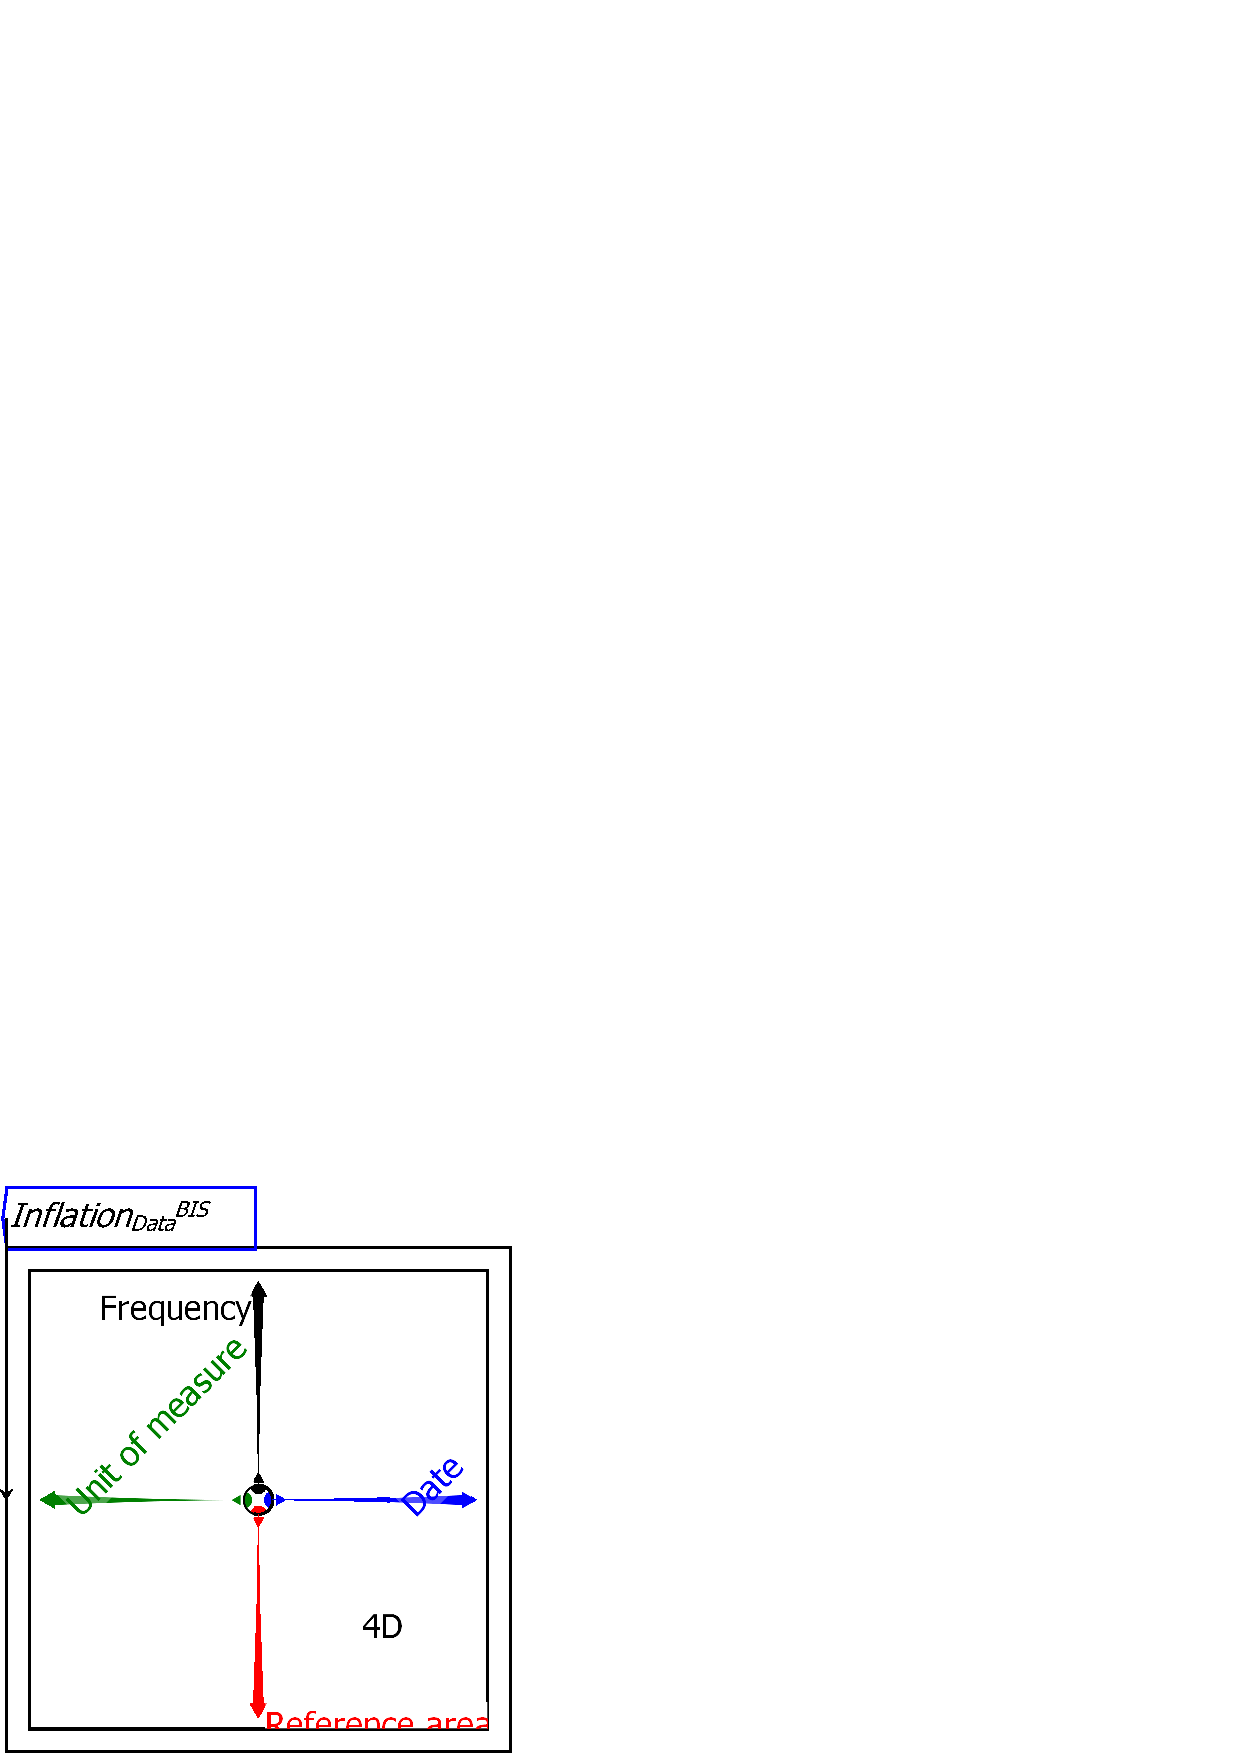
\includegraphics{images/01RavelDataInflation} 
\par\end{flushleft}

There are many ways to manipulate and display data directly from a
Ravel. This is a Ravel with data attached and selected for graphing:
the "Year on Year Changes" data is selected from the Unit of Measure
axis; two countries (Japan and the United States) are selected from
the Reference area axis via the \emph{Pick axis slices} command; Monthly
data is chosen from the Frequency axis; and Calipers are applied to
the Date axis to select data from 1960 till 2024.

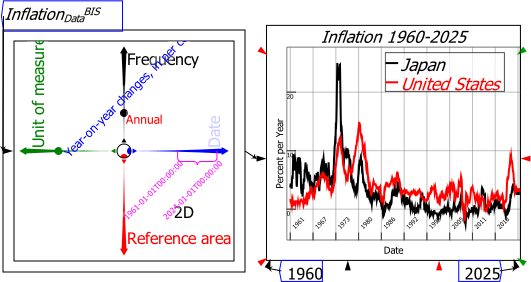
\includegraphics[width=10cm]{images/01BRavelDataInflationSelected}

Ravel the object itself makes it far easier to drill down into and
visualise data than using either a spreadsheet, or the Pivot Tables
that standard Business Intelligence program use.

\emph{Ravel} the program enables easy analysis of data using self-documenting
flowchart formulas.This is a Ravel with data selected--for six countries,
on the annualised monthly inflation rate, for dates from January 2001
till January 2024--and assigned to a variable ("Post2000").
\noindent \begin{flushleft}
\resizebox{10cm}{!}{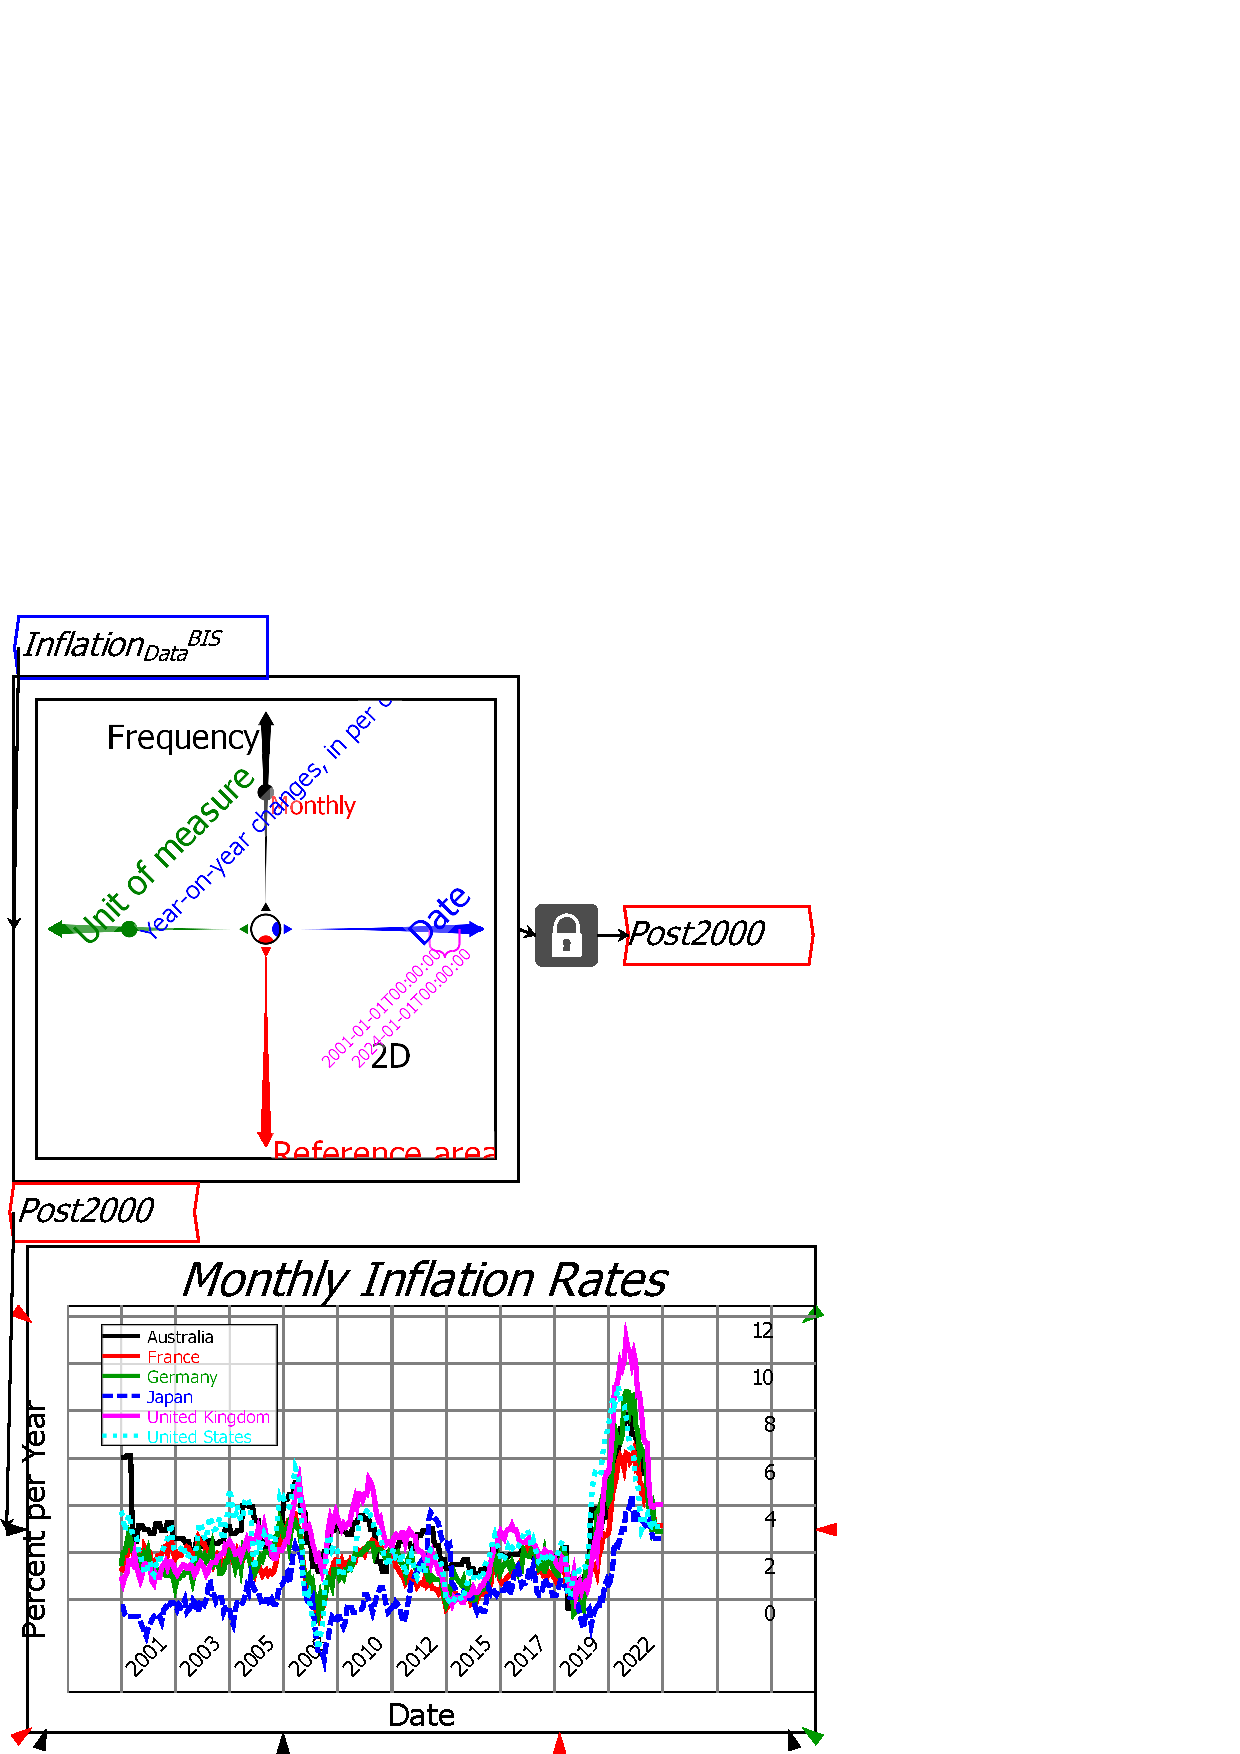
\includegraphics{images/02RavelDataInflationGraphed}} 
\par\end{flushleft}

The data is analyzed by (a) working out the average inflation rate
for the selected countries, and (b) subtracting the average from the
actual inflation rate for each country.

The average inflation rate is calculated using the formula shown below,
where the 
\includegraphics{images/mean}operator works out the average
inflation rate over time for the six countries in the variable \emph{Post2000}
to generate the variable \emph{Inflation}\textsubscript{\emph{Average}}.
This average is then subtracted from the country-specific data in
\emph{Post2000}:

\resizebox{10cm}{!}{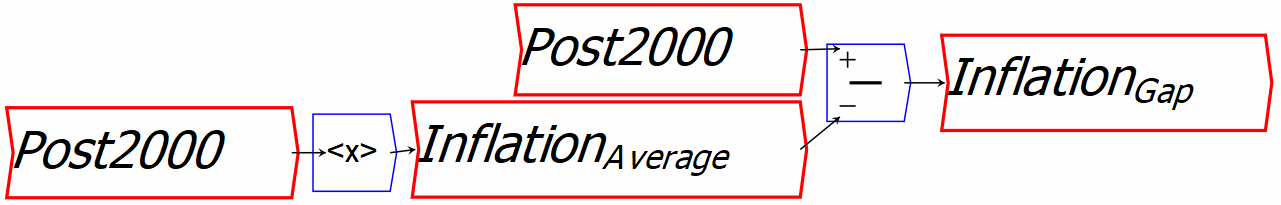
\includegraphics{images/03Formula}} 

This one formula is applied to every country in the Ravel (six countries
in this case) and every quarterly data point (80 quarters). Doing
the same analysis with a spreadsheet would require writing an obscure
cell reference formula and replicating it across 480 cells.

This example shows average inflation outcomes for the six countries,
and the deviation of each of them from the average.
\begin{center}
\resizebox{10cm}{!}{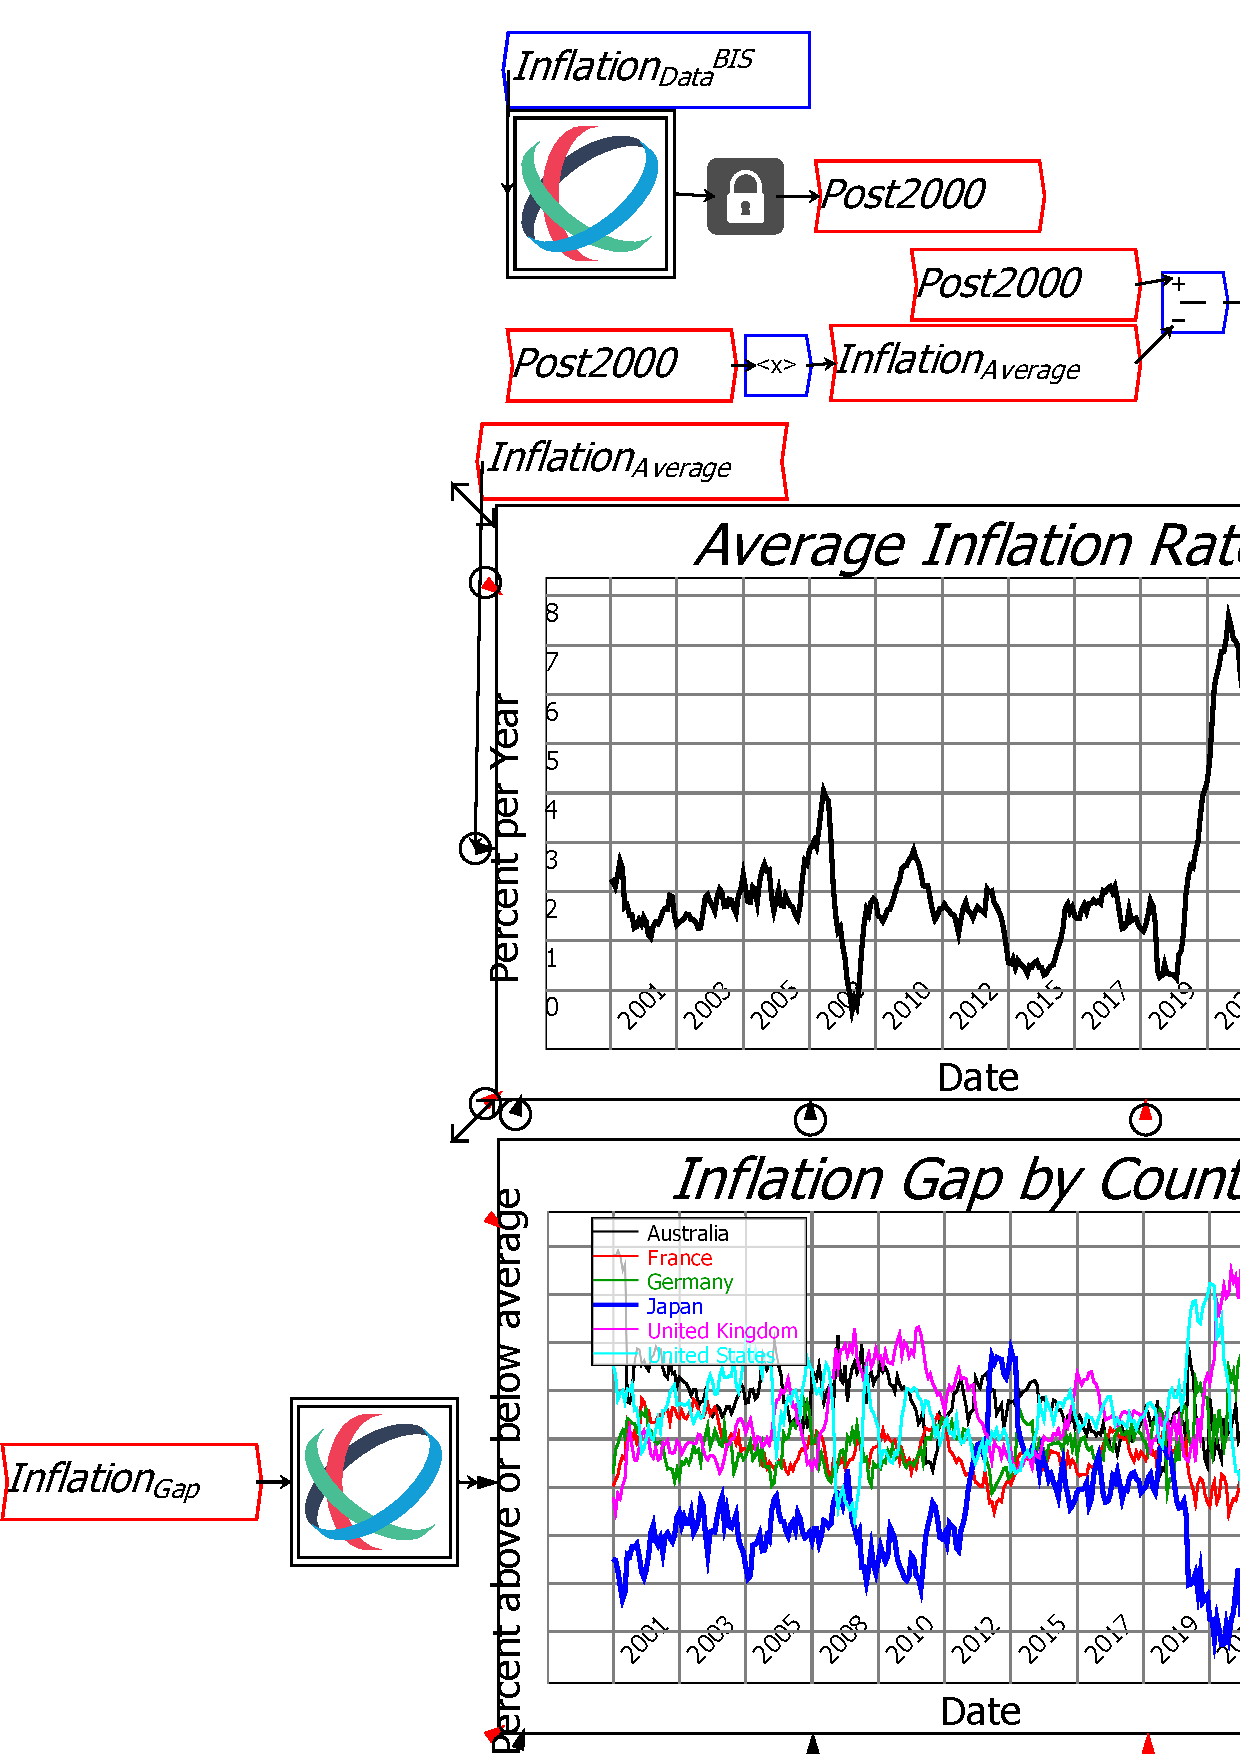
\includegraphics{images/03RavelDataInflationAnalyzed}} 
\par\end{center}

This illustrates the capacity of Ravel to rapidly provide insights
from data--in this case, that the best-performing country during
the post-Covid inflation was Japan, and the worst performing were
the USA and UK. This is noteworthy, because both the USA and UK sharply
increased interest rates with the intention of reducing inflation,
while Japan kept its interest rate constant. Perhaps then, interest
rates aren't effective at controlling interest rates? 

These examples are drawn from economics, mainly because \emph{Ravel}'s
inventor is an economist (and a contrarian one at that). But \emph{Ravel}
can analyze any data you give it---marketing data, scientific data,
production data, whatever. It can also handle enormous data sets,
far larger than are manageable with Excel.

We hope these examples show how easy it is to turn data into information
using Ravel.
